\chapter{相关研究基础}
% 脚注使用带圈数字的表示方法,此处为示例 1\footnote{测试脚注一} 和示例 2\footnote{测试脚注二}。

% 参考文献可以使用\cite{BUPT_Thesis_Format_2014}和\onlinecite{BUPT_Thesis_Format_2004}的表示方法。

\section{段路由}

\subsection{段路由发展历史}

在开放系统互连模型网络架构中,网络层的核心协议IP协议只提供尽全力交付的服务,是无连接、不可靠的,因此网络流量服务的可靠性通常由传输层协议 \gls*{TCP} 来完成。而对于IP层的路由协议来说,如何评估网络的性能以及如何对网络性能进行优化依然是需要考虑的问题。虽然 \gls*{OSPF} 和 \gls*{IS-IS} 等协议定义了路由器之间如何通信以及何时更新链路权重等信息,但它们并不能对网络性能做出评估。为此,一个IP网络层的关键问题就是如何预测或估计网络中的流量状态,以及IP网络如何实现一些业务可能感兴趣的网络性能度量。这就产生了网络流量工程,流量工程是为了处理IP网络的性能评估和性能优化问题 \cite{CNTE} 。流量工程包括了各种应用于网络流量的测量、表征、建模和控制的技术和科学原理。而对于使用网络流量工程的网络工程师来说,流量工程的目标就是通过合适的技术手段获得适当的链路权重来使业务的流量运行在符合其带宽、抖动、时延、丢包率等 \gls*{QoS} 需求的路由路径上。

自从 \gls*{MPLS} 诞生以来,使用 \gls*{MPLS} 隧道技术实现流量工程就是一种最常用的流量工程方法。甚至一提到流量工程,工程师们通常都会着眼 \gls*{MPLS} 来实现流量工程。 \gls*{MPLS} 流量工程需要网络运营商为每条链路分配带宽值。分配的带宽通常等于链路的物理带宽。 \gls*{MPLS} 流量工程还允许为每个 \gls*{MPLS} 隧道分配带宽值。该值通常等于测量的隧道承载的流量。因为链路的分配带宽值和 \gls*{LSP} 由 \gls*{RSVP} 发出信号,这些带宽值通常称为链路和隧道的资源预留协议带宽。在将隧道放置到网络上时, \gls*{MPLS} 流量工程将确保在任何链路上,通过该链路的所有隧道的带宽总和小于该链路的带宽。从概念上讲,这可确保每条链路的带宽都超过所需的带宽,从而防止拥塞。

\gls*{MPLS} 是很成熟的流量工程协议,但是它的问题在于两点,一个是 \gls*{MPLS} 需要规划好一条流量每一跳的目的地址,使得流量十分精确地按照预期的路线传输,这就使得 \gls*{MPLS} 不能很好地绕过网络中随机出现的链路故障,并且完全架空了IP网络天生支持的 \gls*{ECMP} 等负载均衡方式,使得流量工程强依赖于对链路进行精确计算的管理控制设备,缺少自愈的可能;第二点是在于 \gls*{RSVP} 为了对网络带宽作出精确的估算,相当占据网络中的各种资源,尤其是当网络规模日益扩大之后,资源预留协议需要协商的链路及路由器也越来越多, \gls*{RSVP} 的过于冗杂对网络运行造成了比较大的负担。

因此在2015年,思科提出了段路由技术 \cite{SRARK}。段路由是一种相对较新的流量工程方法,在此之前更常用的流量工程技术。段路由的关键思想是将路由路径分解为分段,以便从宏观上更简单地控制路由路径,从而提高网络利用率。为了与现有网络技术兼容实现平滑过渡,段路由技术在提出伊始就准备了两套数据面,一个是于 \gls*{MPLS} 的段路由,一个是基于IPv6的段路由 \gls*{SRv6} 。基于 \gls*{MPLS} 的段路由的段标签在本质可以看做是和 \gls*{MPLS} 标签含义相同的属性,路径上的路由器仍然可以使用 \gls*{MPLS} 传统的推送、弹出和交换操作数据包头的段路由报文头。基于 \gls*{MPLS} 的段路由和基于 \gls*{MPLS} 一样有两种基本类型的段标签:节点标签(Node Segment)和邻接标签(Adjacency Segment)。节点段标识路由器节点,节点段的编号在整个分段路由域中是全局唯一的。邻接段代表节点的本地接口。相邻段编号通常仅在本地有意义在每个节点上。由于可以使用相同的标签交换机制,因此可以利用 \gls*{MPLS} 数据平面基本上无需修改即可实现分段路由。除了与已有网络方案无缝过渡外,段标签使用对当前域内路由协议的简单扩展以在整个网络中分发,因此分发标签不再需要 \gls*{LDP} 和 \gls*{RSVP-TE} ,可以显着简化控制平面的协议和流量。此外,段路由与 \gls*{MPLS} 技术不同的是,除了在入口节点上,不需要在分段路由中维护路径状态,因为现在数据包是根据它们携带的分段列表进行路由的。而数据包的修改必须在入口节点完成,因为入口节点需要确定段路由策略并将分段标签添加到数据包中。

一个基本的段路由实现首先需要入口节点在数据包的IP头上添加一组段路由节点标签,每个标签指向一个段路由节点,这些标签会用作每一段路由中的临时目的地址,沿途的非目的地址交换机就会使用标准最短路径路由算法路由数据包。然后当数据包从入口到达中间目的地时,中间目的地弹出栈顶标签,现在数据包再次沿着最短路径从中间节点路由到下一个段路由节点。最后当报文到达段列表里最后一个节点时,该节点会弹出整个段路由报文头。

一个$n$段的段路由路径被称n-段路由($n-segment$)。如果可以允许任意数量的段,段路由就可以衍生使用任意路径,因此在一个路由段数不被限制的n-段路由问题中,在段路由网络中生成段路有航点列表就可以被视为解决多商品流问题。这种灵活性是以增加标签开销和增加网络中的标签处理为代价的。从流量工程的角度来看,不使用最短路径路由的大部分收益都可以通过使用两跳段路由来实现。实验研究表明 \cite{SIDLENGTHANALYSIS, SIDLENGTHPROVE} ,2-段路由的表现几乎与完全不限制段路由长度的解决多商品流问题一样好。因此,本文会关注使用本文提出算法的2-段路由的表现,即其中入口和出口之间的流量只通过一个中间段路由节点。本文中开发的相同技术可以扩展到具有2个以上段的段路由,但是这确实会造成计算量增加代价。除了段路由列表的长度外,在段路由问题中控制平面也起到了很大的作用,因此研究控制平面如何为每个流选择合适的段路由策略才能以最大限度地减少整体网络拥塞也是一个常见的段路由研究方向。

对于段路由研究领域的类别,Ventre \cite{SRSURVEYS} 等的研究提出了一个比较全面的分类方式,它是基于对七个主要研究类别段路有研究领域分类。第一个是监控类,收集所有描述和实现与网络监控活动相关的工具研究,这其中包括测量给定输入路线上的端到端延迟或评估流量。第二类是流量工程,包括所有提出高级路由策略以优化网络性能的工作。第三类是故障恢复,涵盖在节点/链路故障的情况下提供快速网络恢复的解决方案。由于时间尺度的限制,这一类的工作是基于本地机制的,即不涉及集中式控制器。第四类是集中控制架构,包括所有侧重于在底层网络(IP网络、软件定义网络、 \gls*{MPLS} 网络)之上实现集中控制平面的段路由网络实施的研究。在这里需要指出,尽管一些归类为流量工程的工作是基于集中控制的架构,但它们不包括在集中控制的架构中类别。这是因为它们的主要范围仍然是优化流量工程目标(例如减少拥塞或最小化能源消耗)。在路径编码类别中,研究将所有提出旨在将网络路径转换为段路由列表的算法的论文分组。具体来说,研究将通用路径编码算法提供的一系列节点和链接形式的路径作为输入,将在数据包头中推送的段路由编码序列作为输出,以便引导数据包沿着输入路径转发。第六类是网络编程,包括利用段路由的可编程性特性的解决方案的研究成果,即构造基于服务的段路由编码来定义数据包即将穿过的特定段列表,服务功能链相关的研究就属于属于这一类别。

\subsection{段路由模型}

段路由的数据平面定义了如何对段路由节点以及支持段路由的服务节点等网元进行编码,并定义了段路由的转发语义,即每个设备应如何基于分段处理数据包。段路由的控制平面则是定义了段标识符如何在网络设备之间传播,以及如何指示网络设备在流上应用给定的段列表。

1. 段路由数据面

从抽象的角度来看,段路由头包含一个段列表,以及一个指向数据包活动段的指针,是处理数据包的设备需要执行的指令。当活动段被执行后,列表中的下一个段成为活动段。 \gls*{SID} 是段的标识符。根据其类型,段路由编号可以具有域范围的意义,也可以仅对处理它的路由器在本地有意义。

段标签的类型通常有:与节点关联的、路由器分配时需要确保一个域范围的唯一的节点段标签(Node SID)或前缀标签(Prefix SID),通常由网络工程师手动完成,或使用中央控制器分配完成;每个路由器将为它的每个 \gls*{IGP} 邻居分配的一个仅本地有效的邻接段标签(Adjacency SID);标记网络中可以提供指定服务节点的服务段标签(Service SID),各个段标签的类型及其用途如图2-1所示。

\begin{figure}[htbp]
\setlength{\abovecaptionskip}{15pt plus 3pt minus 2pt}
\centerline{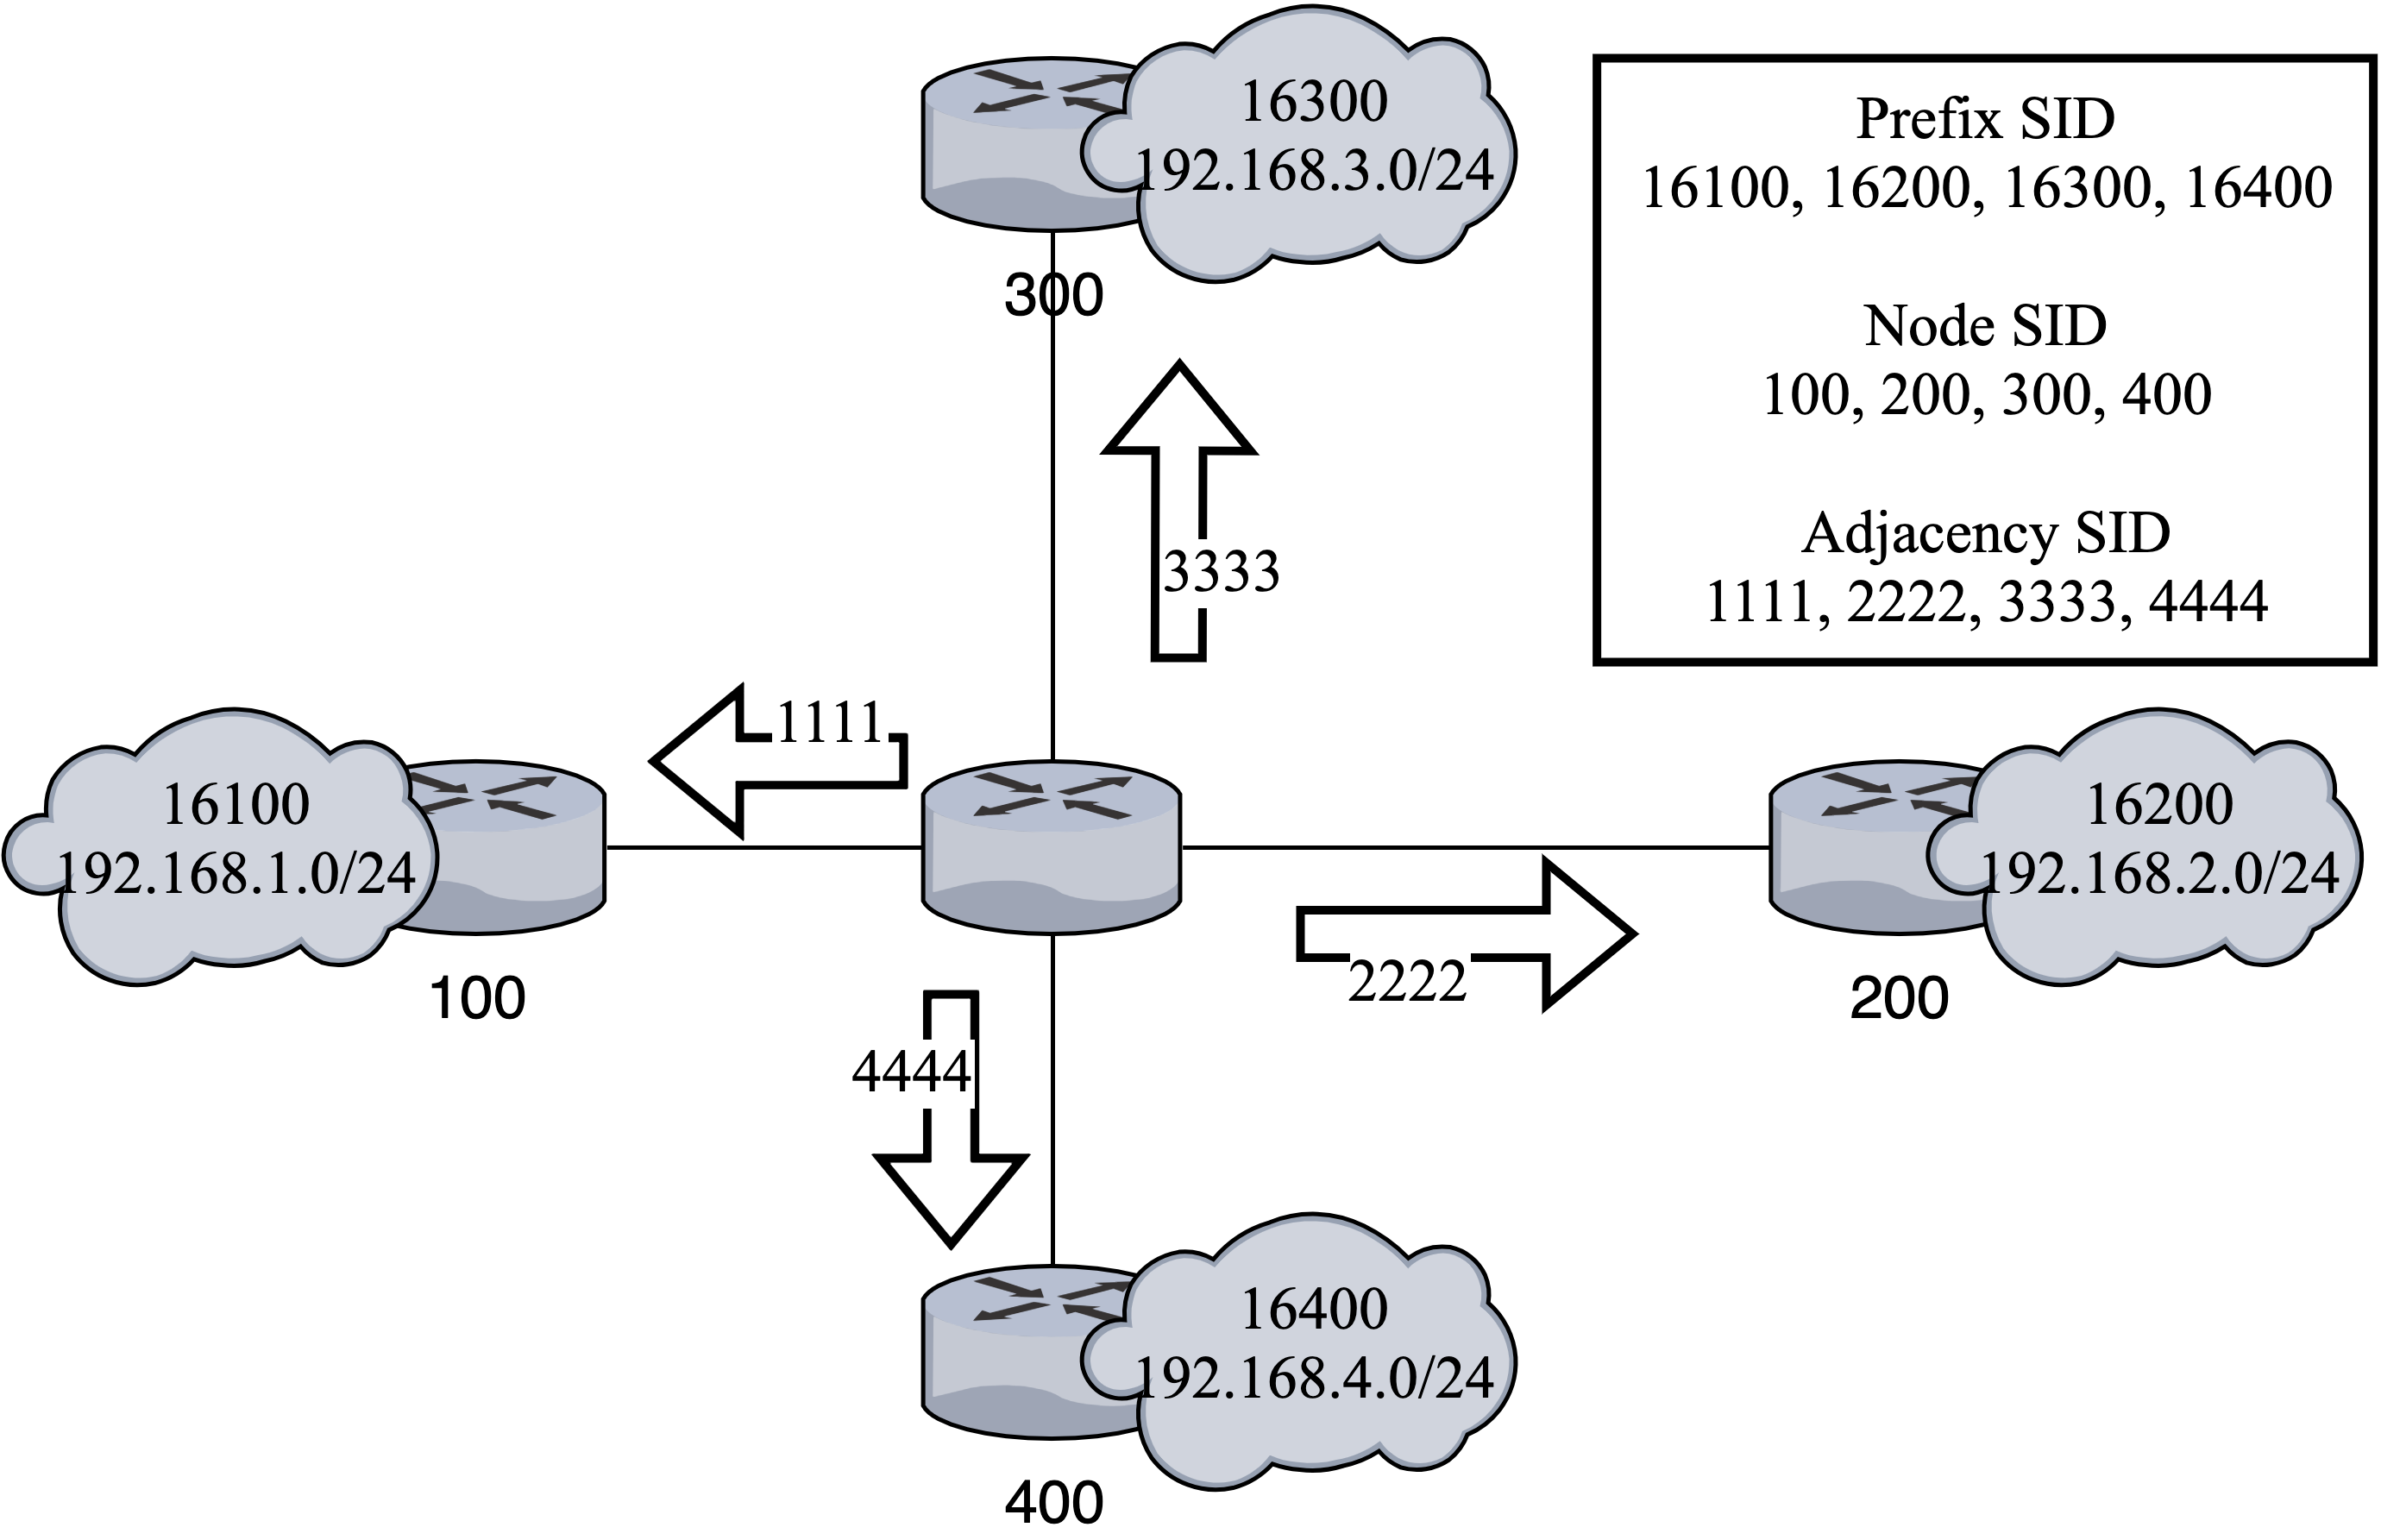
\includegraphics[width=0.9\textwidth]{./figures/ch2-kinds-of-SID.png}}
\caption{段标签的类型及其用途示意图}
\label{fig-ch2-kinds-of-SID}
\end{figure}

段路由节点通常支持以数据平面下操作:基于活动段执行的转发的CONTINUE操作;在数据包的段路由报文头之前添加一个段,并将该段设置为活动段的PUSH操作;以及将下一个段标记为活动段NEXT操作 \cite{SRARK} ,如图2-2所示。

\begin{figure}[htbp]
\setlength{\abovecaptionskip}{15pt plus 3pt minus 2pt}
\centerline{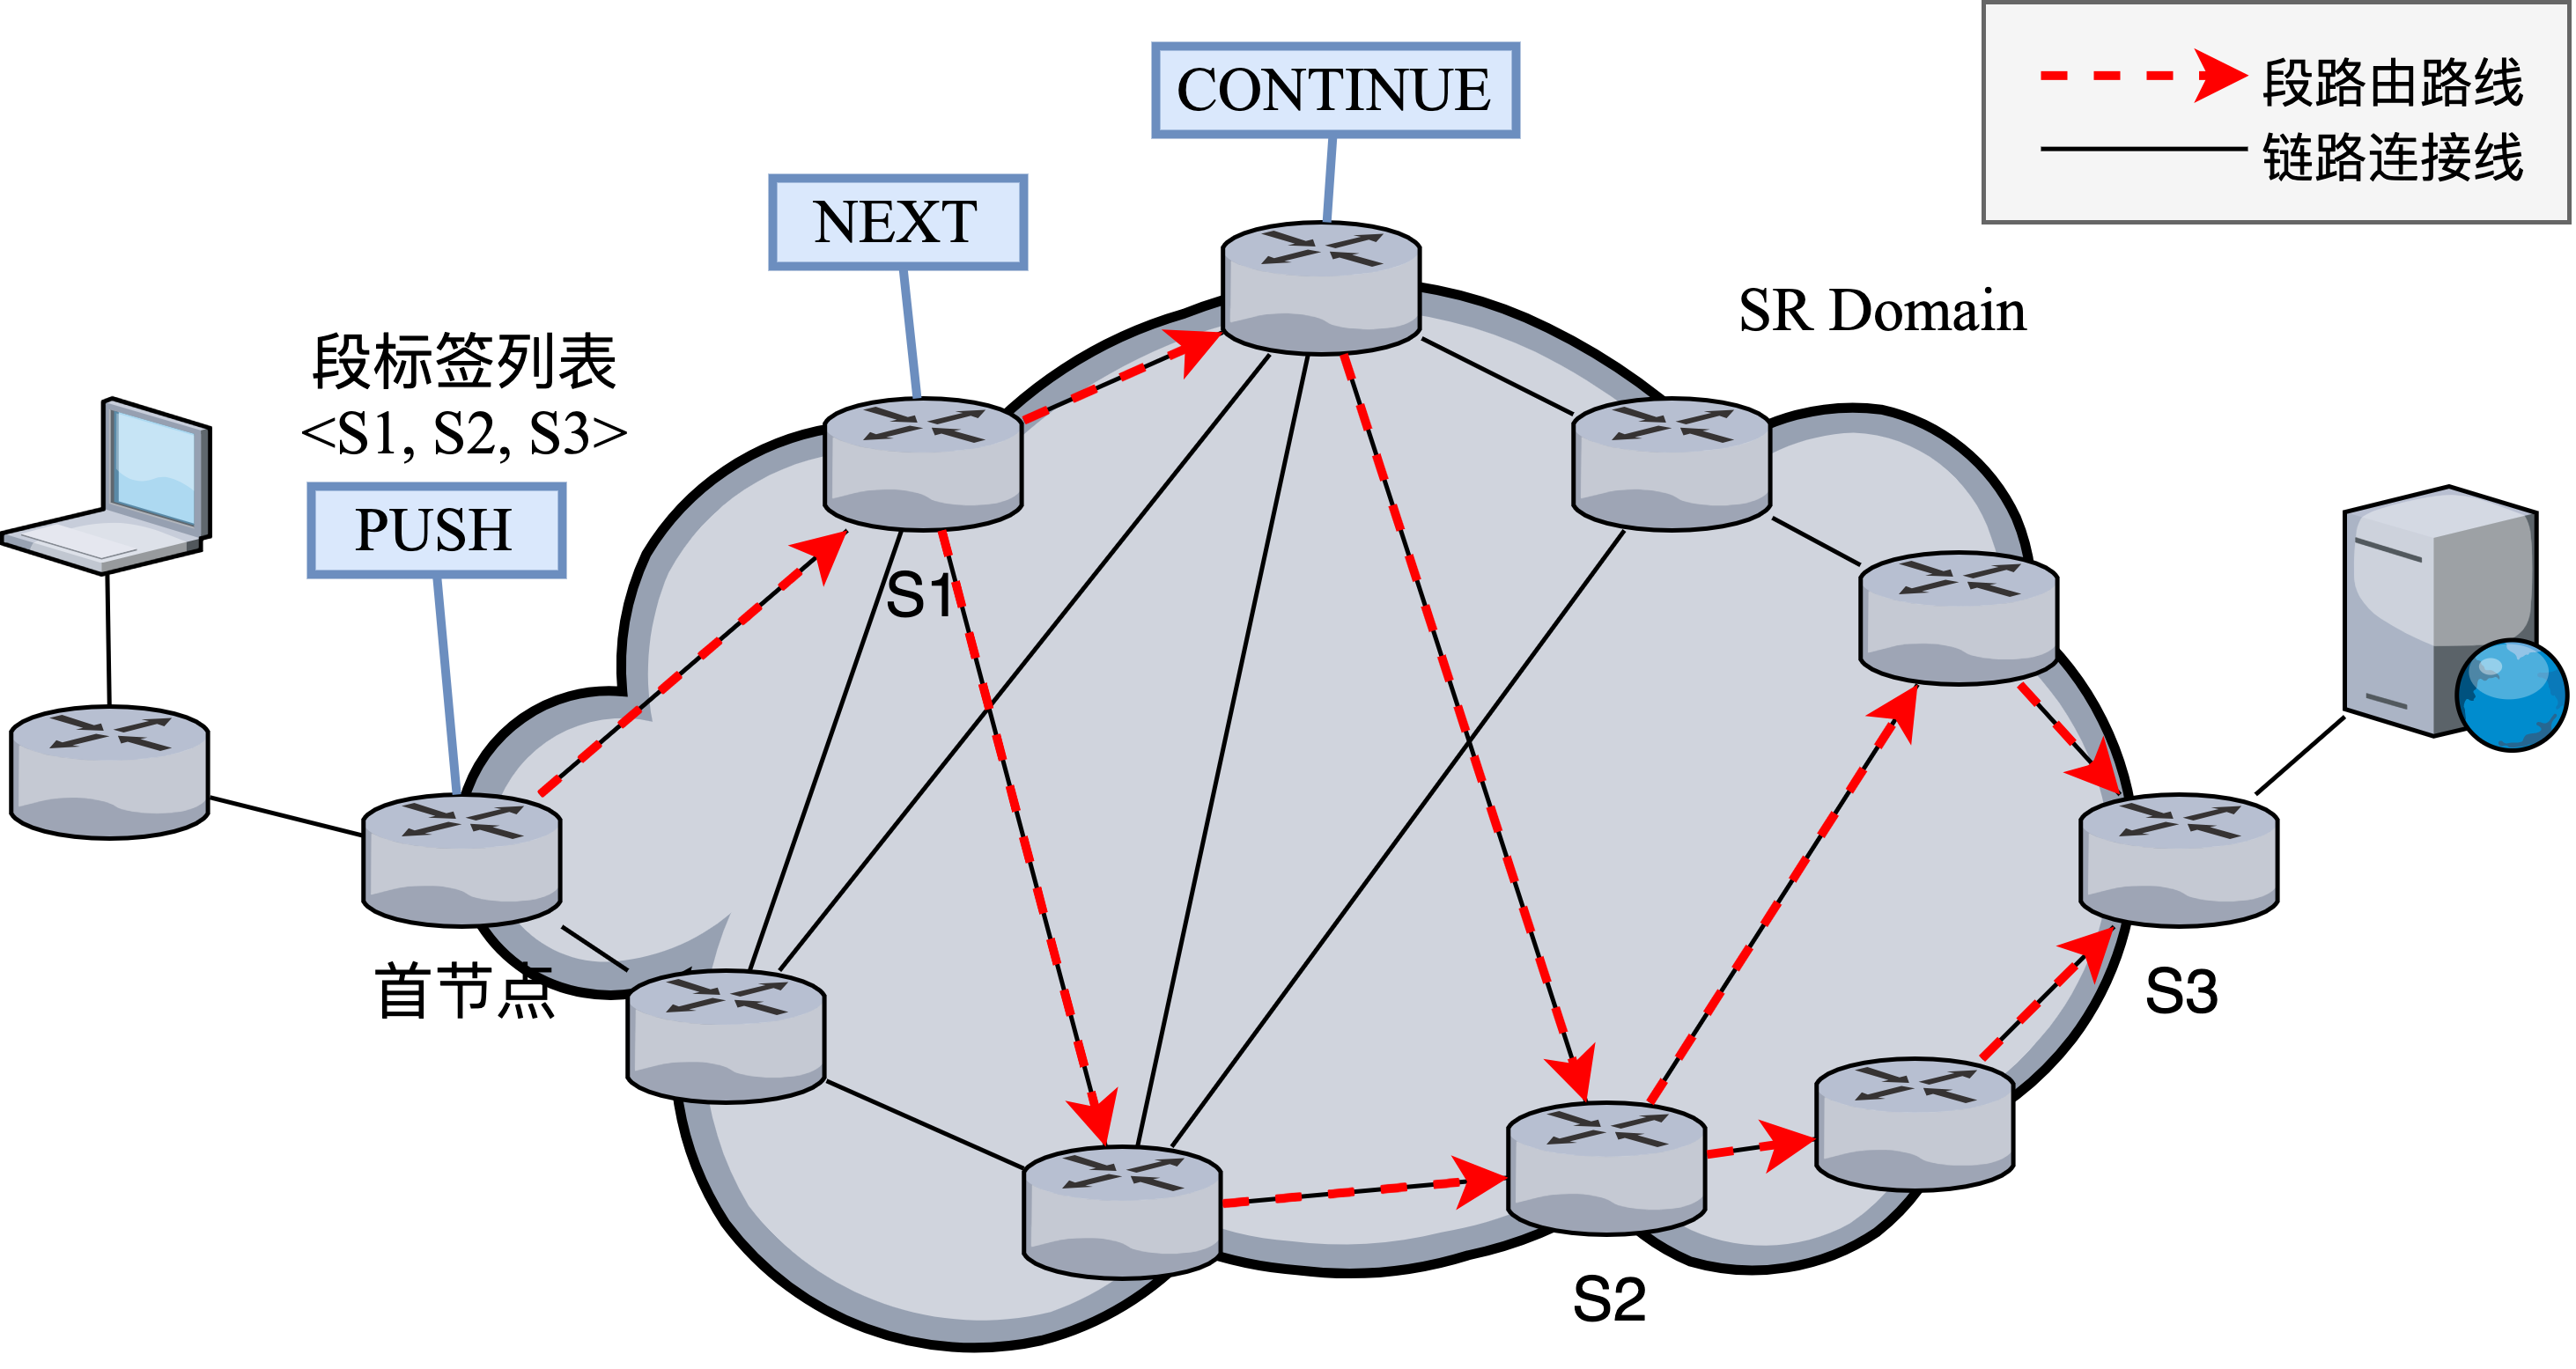
\includegraphics[width=0.9\textwidth]{./figures/ch2-SR-actions.png}}
\caption{段路由节点操作示意图}
\label{fig-ch2-SR-actions}
\end{figure}

如上文所提到,段路由主要有两种数据面类型, \gls*{SRv6} 和基于 \gls*{MPLS} 的段路由(SR-MPLS)\cite{SRMPLS}  ,两种数据面功能相似但又有很多不同,功能对比如表2-1所示, \gls*{SRv6} 在网络编程上有很大的优势,但是由于其不随路弹出标签的特点和IPv6地址占资源较大的特点,在协议开销、带宽承载效率和 \gls*{MTU} 以及硬件处理效率等资源需求很大,因此现在有一些研究 \cite{GSID, MICROSID, USID} 也着眼于压缩段路由报文头,例如uSID \cite{USID} 只包含MPLS的20bit的段标签信息的优化方案。

\begin{table}[]
\resizebox{\linewidth}{!}{
\begin{tabular}{|l|l|l|}
\hline
数据面方案 & SR-MPLS &  \gls*{SRv6}  \\ \hline
协议开销 & 4*5=20B & \begin{tabular}[c]{@{}l@{}}16*4\textasciicircum{}2(Segment 列表)+8B(SRH)\\ +40B(IPv6 报头)=112B\end{tabular} \\ \hline
有效负载承载效率 & 440/(20+440)=95.7\% & 440/(112+440)=79.7\% \\ \hline
MTU & 1520B & 1612B \\ \hline
\begin{tabular}[c]{@{}l@{}}对硬件\\ NPU/ASIC 要求\end{tabular} & \begin{tabular}[c]{@{}l@{}}最多只需读出前 20B(标签栈)\\ +20B(IPv4 报头,用于负载均衡)\\ 报头信息即可转发。执行的操作是 \\ SR-MPLS 定义的标准“压入”、\\ “交换”和“弹出”标签操作\end{tabular} & \begin{tabular}[c]{@{}l@{}}需要读出前 112B 报头信息才能\\ 转发执行的操作类型接近 20 种,\\ 包括Underlay、Overlay 和服务\\ 编程等,并且还在不断扩展之中\end{tabular} \\ \hline
\begin{tabular}[c]{@{}l@{}}转发过程是否弹出\\  Segment\end{tabular} & \begin{tabular}[c]{@{}l@{}}弹出。栈顶标签即为活动\\ Segment\end{tabular} & \begin{tabular}[c]{@{}l@{}}不弹出。通过 Segment Left 指针\\ 标识出活动 Segment\end{tabular} \\ \hline
负载均衡实现 & \begin{tabular}[c]{@{}l@{}}一般根据净荷的 IP 5 元组进行哈希;\\ 如果 Segment 数量多,需要使用\\ Entropy 标签\end{tabular} & \begin{tabular}[c]{@{}l@{}}根据外层 IPv6 报头的 Flow Label\\ 字段进行哈希\end{tabular} \\ \hline
\begin{tabular}[c]{@{}l@{}}对网络中间航路点\\ (非头端)的要求\end{tabular} & \begin{tabular}[c]{@{}l@{}}低。由于 SR-MPLS 的开销小,\\ 而且会逐步弹出,因此中间节点\\ 查找的难度不大。主要的挑战\\ 在于在标签栈数量多时,如何\\ 实现有效的负载均衡\end{tabular} & \begin{tabular}[c]{@{}l@{}}高。由于  \gls*{SRv6}  不弹出 Segment,\\ 因此即使是中间航路点,也需要\\ 读取整个  \gls*{SRv6}  报头。\end{tabular} \\ \hline
\end{tabular}}
\caption{SR-MPLS和SRv6区别整理表}
\label{table-SR-MPLS-SRv6}
\end{table}

2. 段路由控制面

段路由的控制平面定义了段路由编码的数据包如何在网络设备之间进行通信。在段路由网络中,节点段编码和邻接段编码将通过内部网关协议进行通告。 \gls*{IS-IS} 和 \gls*{OSPF} 是服务提供商网络中最流行的内部网关协议,它们被扩展为支持分段编码的通告和分配。内部网关协议的扩展将允许任何路由器维护所有节点和邻接段的数据库。此外,通过利用这两个内部网关协议的亚秒级收敛特性,可以在任何拓扑更改后快速更新每个路由器上的段路由数据库。请注意,使用这些扩展,就可以在网络中执行端到端封装而无需启用和管理其他协议,例如标签分发协议。

段路由控制平面的另一个元素涉及如何指示入口路由器选择数据包应遵循的段路由航点列表。为此,可以使用以下方法:

\begin{itemize}
\item 分布式 \gls*{CSPF} 计算方法。在这种方法中,入口路由器计算目的地的最短路径,条件是该路径符合某些标准。然后计算对这条路径进行编码的一系列节点和邻接段;
\item 基于软件定义网络控制器的方法。段路由提供了一个可扩展和有弹性的数据平面,同时允许软件定义网络环境通常假设的控制灵活性。这方面导致计划在一些面向软件定义网络的控制器设计中支持段路由。例如,Open Daylight控制器 \cite{ODL} 支持使用 \gls*{PCEP} 控制段路由,如图2-3所示。另外,段路由隧道的静态配置可能用于特定目的,例如测试或故障排除,但由于明显的可扩展性、弹性和管理限制,通常不建议将其用于长期网络操作。
\end{itemize}

\begin{figure}[htbp]
\setlength{\abovecaptionskip}{15pt plus 3pt minus 2pt}
\centerline{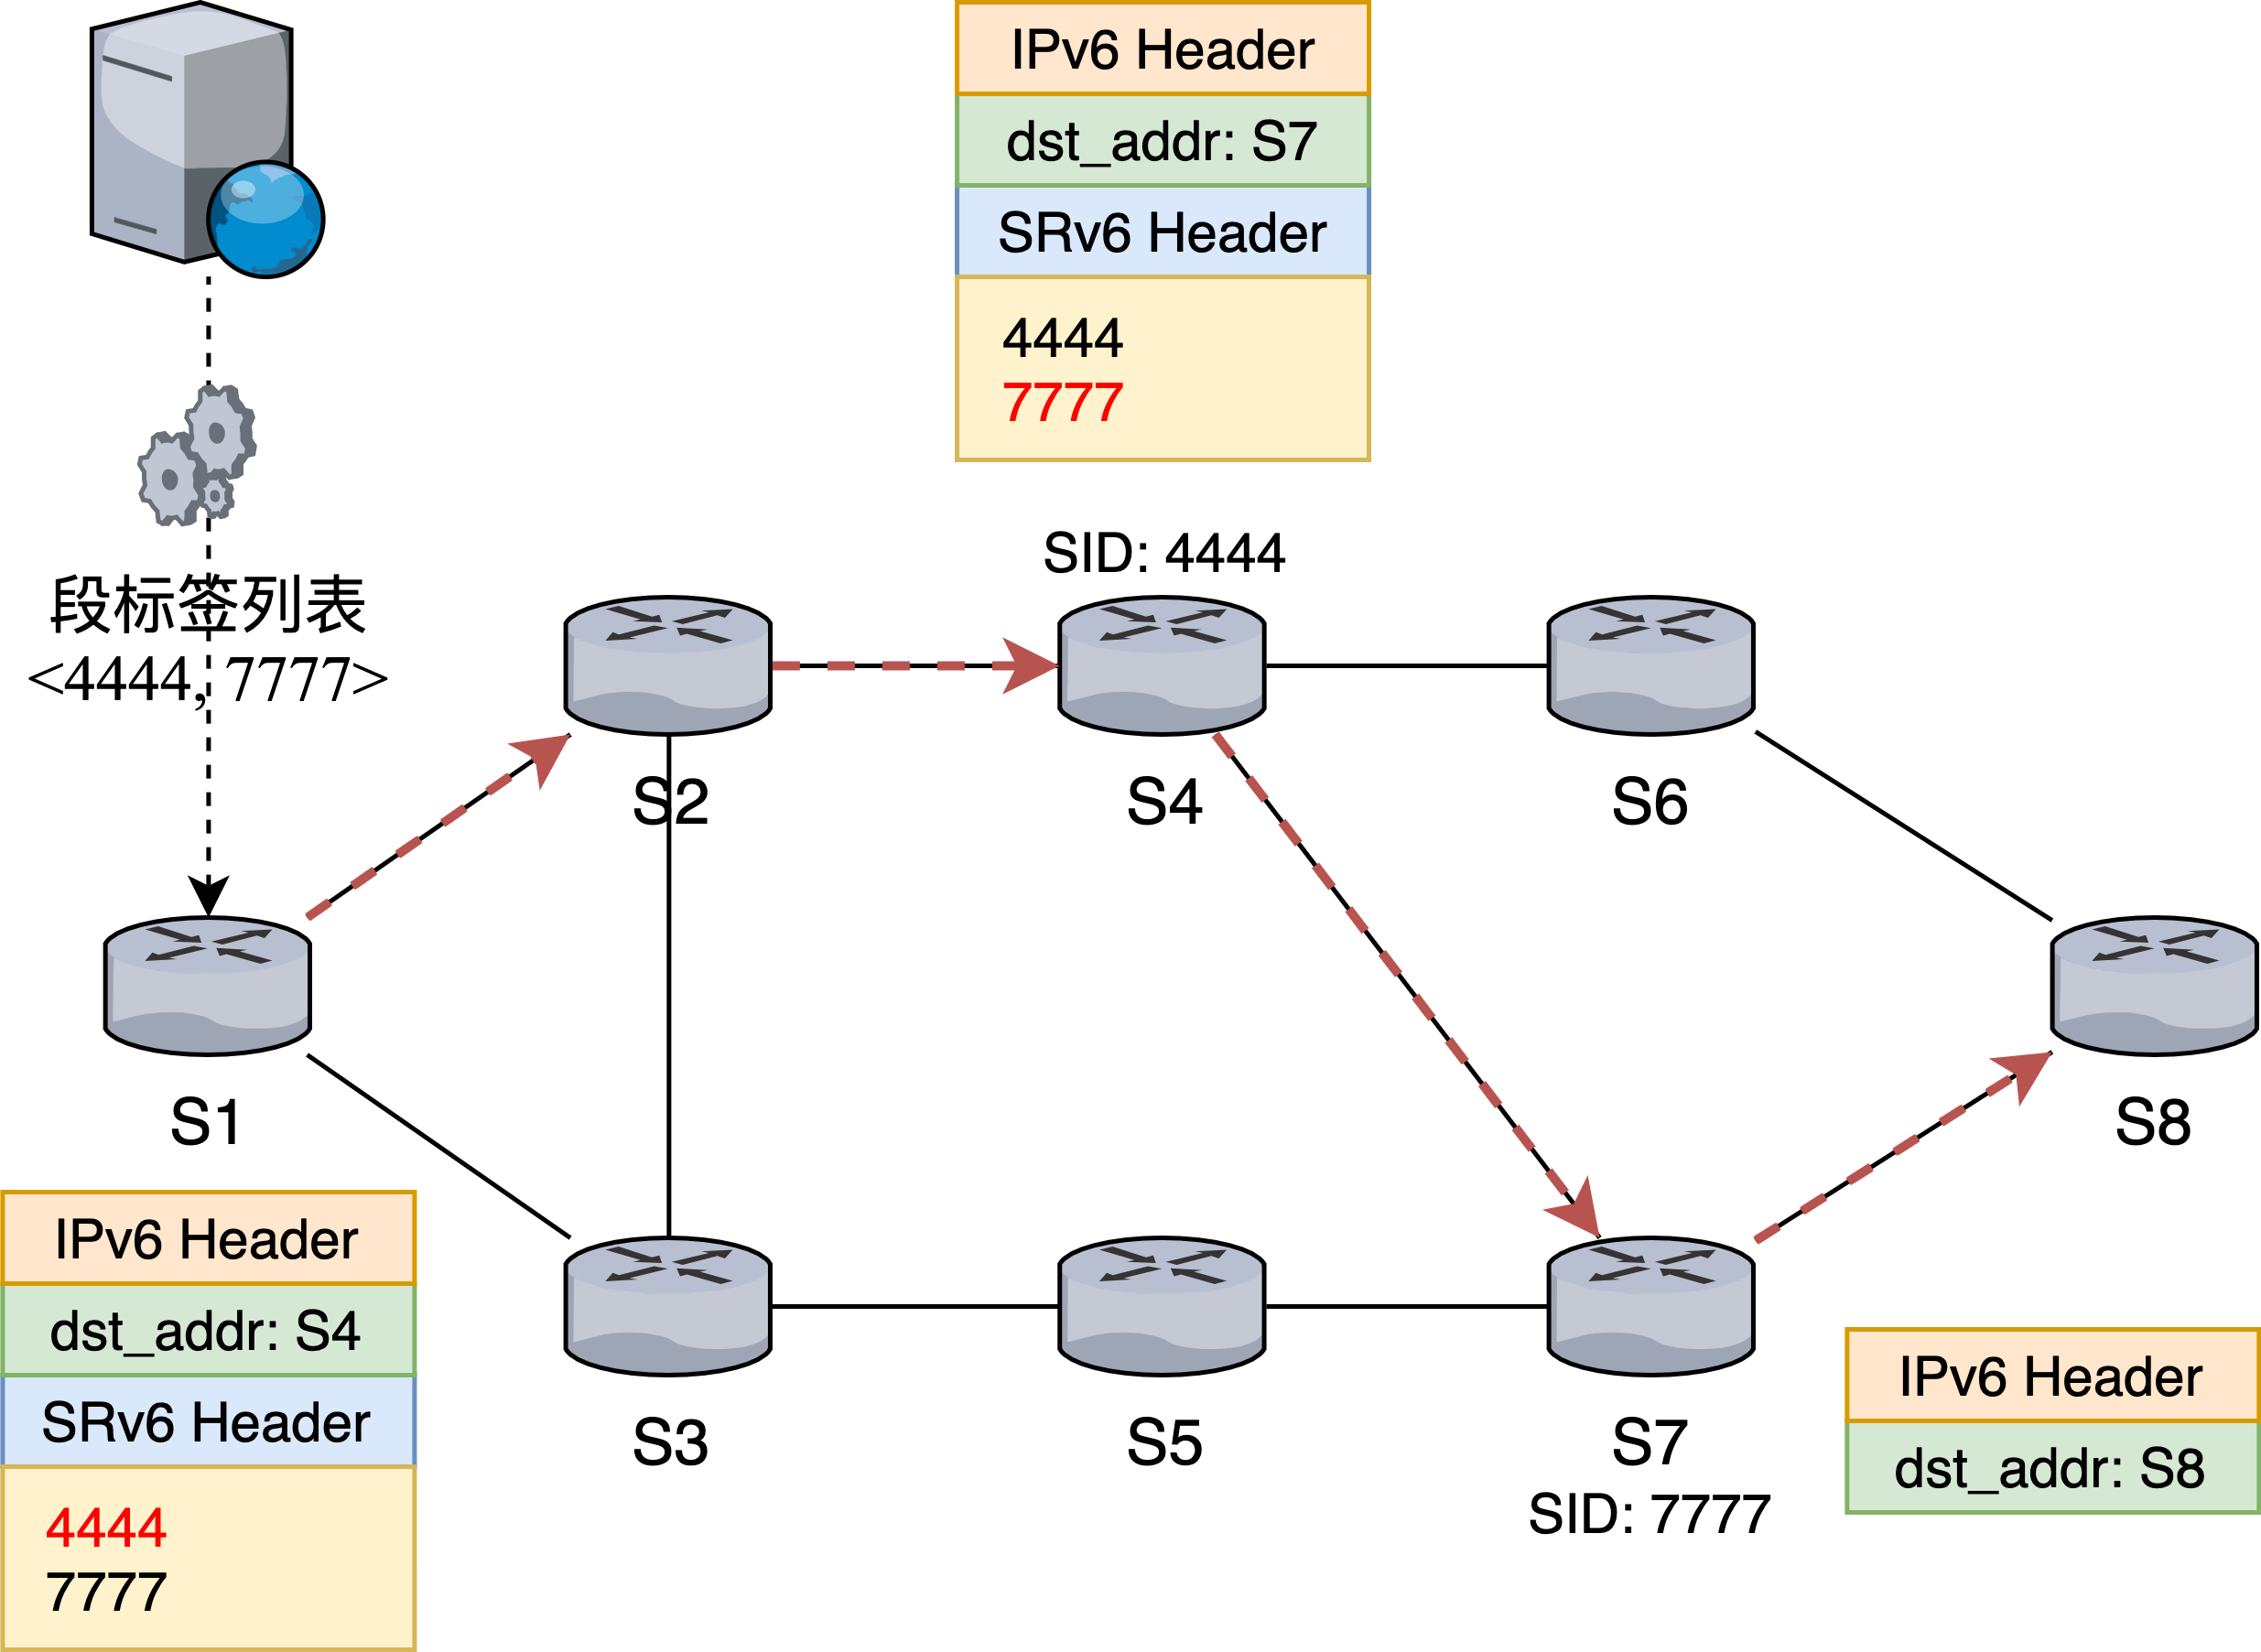
\includegraphics[width=0.9\textwidth]{./figures/ch2-sr-model.png}}
\caption{集中式控制面段路由模型}
\label{fig-ch2-sr-model}
\end{figure}
    
综上所述,段路由控制面可以支持集中式的控制器的标签分发和规则制定,也可以支持分布式的基于域内网关协议和域间网关协议的标签配置,两者的选择可以根据网络的具体情况来制定。

3. 段路由流量工程研究

段路由具有对于普通流量不指定路径进行自动负载,对于需要调度的流量计算出显式路径,并下发段路由策略来指导交换机执行的优势。段路由支持网络编码的特点在路由灵活性方面也具有格外吸引人的优秀特性,因此段路由被广泛用于流量工程服务保障相关的问题。一些调查显示 \cite{SRSURVEYS} ,有多篇论文利用段路由来提供先进的流量工程解决方案。流量工程的研究工作通常都采用优化问题的经典模型结构:第一必须最小化/最大化目标函数,第二从模型中抽象出一组值得考虑的参数,以及第三考虑特定的网络场景。调查的文献中通常涵盖了三个不同的流量工程目标,即最小化网络能耗、优化拥塞和最小化被拒绝请求的数量。段路由与使用最短路径算法的协议有一个显著不同的地方在于段路由允许的高灵活性的路由路径,这可能会导致数据包在转发中出现复杂而冗长的网络路径。因此,段路由技术在根据特定目标优化段路由航点列表的同时,重要的是要考虑过于复杂的路由解决方案可能对网络性能,如吞吐率产生的影响。除了端到端延迟之外,一些审查的工作还考虑了与段路由相关的开销,包括由于插入段路由报文头的数据包而浪费的带宽,以及要配置段路由转发策略的边缘路由器的数量。最后,还有一些研究着重对网络部署情况进行讨论,所考虑的网络可以是完整的段路由网络,即所有节点都具有段路由能力,也可以是部分节点部署段路由技术的网络,后者中只有一部分节点可以处理段路由报文头,其他节点只能按照网络层协议进行浅层次的转发。由于在数据包中插入段路由报文头而浪费的带宽,以及要在边缘路由器中配置的段路由转向策略的数量。最后,所考虑的网络可以是完整的段路由网络,即所有节点都具有段路由能力,或者是部分部署的段路由,其中只有一部分节点可以处理段路由报文头。

\section{时延研究}

如今,越来越多的应用和平台对低延迟的要求越来越高。然而,在提供低延迟路由服务的广域网中开发新的路由协议非常具有挑战性,并且由于兼容性、可行性、可扩展性和效率方面的障碍,仍然是一个悬而未决的问题。时延相关研究在数据链路层和传输层已经有了很多的研究进展,例如时延敏感网络。由于以太网通信基于尽力而为原则,以太网网络中的数据交换缺乏确定性。到目前为止,以太网中的确定性数据交换只能通过专有解决方案实现,但时间敏感网络旨在改变这种状况。时间敏感网络是一项即将推出的新技术,其重点是通过设计使以太网具有确定性。时间敏感网络是指一组IEEE 802标准,默认情况下使以太网具有确定性。时间敏感网络是一项即将推出的新技术,它位于开放系统互连模型网络架构的第2层。它添加了定义以保证以太网网络中的确定性和吞吐量 \cite{TSN1, TSN2, TSN3} 。以下是构成时间敏感网络的一些 IEEE 标准:增强的同步行为(IEEE 802.1AS)、暂停(抢占)长帧(IEEE 802.1-2018)、计划流量的增强功能(IEEE 802.1Q-2018)、路径控制和带宽预留(IEEE 802.1Q-2018)、无缝冗余(IEEE 802.1CB)、流预留(IEEE 802.1Q-2018)。总而言之时间敏感网络源自业界对音频/视频传输的使用以及对更多设备和同步通信的需求。网络上的设备比以往任何时候都多,共享和分析的信息也更多。因此,以太网必须表现得更好是有道理的。

同样,网络层作为数据中心、运营商提供服务的重要组成部分,提供更好保障时延的服务也是重要的研究方向,和时间敏感网络这种数据链路层技术不太一样,时间敏感网络可以通过对硬件功率的调整完成无排队的数据链路层网络环境,但是网络层的IP协议已经无法对硬件作出过多干涉,因此需要在IP层独特的技术上作出时延保障优化,而众所周知IP网络层最重要的技术是提供分组交换,分组交换的重要基石就是路由算法。路由算法在很长一段时间一直是基于带宽用最短路径算法进行路由分配的,考虑将时延信息加入各种路由算法是值得考虑的地方。

\section{带内遥测}

随着软件定义网络和可编程数据平面技术的发展,带内网络遥测应运而生。带内网络遥测技术通过业务报文逐跳收集网络状态信息,实现网络服务的端到端可视化。带内网络遥测利用数据平面直接驱动网络测量过程,颠覆了传统网络测量将网络交换设备视为中间黑匣子的研究思路。带内网络遥测技术具有编程灵活、实时性强、噪声小、路径级网络状态感知等优点,已成为网络遥测技术的新兴代表,受到学术界和工业界的广泛关注。带内遥测可以用于测量交换机提供的各种信息,例如带宽、时延、排队队列等。

在带内遥测采集单向时延的研究 \cite{INTSURVEY} 上,Kim \cite{KIM} 等结合带内遥测路径定位信息和交换机排队时延信息,实现基于 \gls*{HTTP} 应用的瞬时时延测量;Mizrahi \cite{MIZRAHI} 等使用少量的比特来标记业务数据包,遥测服务器计算网络的逐跳延迟;Riesenberg \cite{INTRIE} 等基于Marvell的Prestera芯片和 \gls*{P4} 编程语言,采用双标记测量时延使得时延误差小于100纳秒,丢包率测量误差几乎为零;IntMon \cite{INTMON} 等基于 \gls*{ONOS} 控制器和 \gls*{P4} 的 \gls*{BMv2} 软件交换机的对使用 \gls*{UDP} 封装带内遥测进行了尝试并实验验证其有效性。而在在带内遥测采集双向时延的研究上,Pingmesh \cite{PINGMASH} 通过主动 \gls*{Ping} 操作检测数据中心网络延迟变化实现双向带内遥测数据的采集。EverFlow \cite{EVERFLOW} 则发送探测以测试和确认潜在的网络故障,已经经常用于数据中心网络的数据包级网络遥测系统。

因此可见对时延数据进行带内遥测的技术已经相当成熟,时延也逐步取代带宽成为网络中更值得关注的网络服务性能类型。这在拥塞控制技术中已经得到了相当多的应用。例如谷歌2020年获得的Sigcomm最佳论文的Swift模型 \cite{SWIFT} 中就使用的主要拥塞信号就是时延,因为它满足了工程师对拥塞感知的所有要求。谷歌在Swift这篇论文中指出,网络往返时延可以使用现代硬件精确测量,并且它提供了多位拥塞信号,即它不仅对拥塞的状态进行编码,而且对拥塞的程度进行编码。Swift进一步分解了端到端往返时延,以将架构与主机问题分开;通过结合网卡硬件中的时间戳和基于轮询的传输(如Pony Express),它使延迟测量更加精确。Swift使用多个网卡和主机时间戳来分离延迟的组成部分,并进而将网卡收方向数据包延迟和处理时间相加以获得全程排队时延,并通过 \gls*{ACK} 数据包上的报文头将此延迟反映给发送方。

因此使用带内遥测技术作为时延采集的方式是可行的,本研究在后文中不对带内遥测做过多分析,只是使用这一项技术作为时延信息采集的渠道。在实验验证阶段也是采用符合逻辑的遥测方式获取时延。

% 测试所有参考文献类型\cite{CITATION_BOOK,CITATION_ARTICLE,CITATION_PROCEEDINGS,CITATION_INPROCEEDINGS,CITATION_TECHREPORT,CITATION_STANDARD,CITATION_PATENT,CITATION_NEWSPAPER,CITATION_ELECTRONIC,SRSURVEYS}。

%% 本章参考文献
\ifx\usechapbib\empty
\nocite{BSTcontrol}
\setcounter{NAT@ctr}{0}
\bibliographystyle{buptgraduatethesis}
\bibliography{bare_thesis}
\fi
